\documentclass[12pt]{article}
\usepackage{amsmath} % AMS Math Package
\usepackage{bm}
\usepackage{amsthm} % Theorem Formatting
\usepackage{amssymb}    % Math symbols such as \mathbb
\usepackage{graphicx} % Allows for eps images
\usepackage[dvips,letterpaper,margin=1in,bottom=0.7in]{geometry}
\usepackage{tensor}
\usepackage{amsmath}
\usepackage{siunitx}
\usepackage{physics}
\usepackage{amsmath, amssymb, graphics, setspace}

\newcommand{\mathsym}[1]{{}}
\newcommand{\unicode}[1]{{}}

\newcounter{mathematicapage}

\newtheorem{p}{Problem}
\usepackage{cancel}
\newtheorem*{lem}{Lemma}
\theoremstyle{definition}
\newtheorem*{dfn}{Definition}
 \newenvironment{s}{%\small%
        \begin{trivlist} \item \textbf{Solution}. }{%
            \hspace*{\fill} $\blacksquare$\end{trivlist}}%

\makeatletter
% we use \prefix@<level> only if it is defined
\renewcommand{\@seccntformat}[1]{%
  \ifcsname prefix@#1\endcsname
    \csname prefix@#1\endcsname
  \else
    \csname the#1\endcsname\quad
  \fi}
% define \prefix@section
\newcommand\prefix@section{}
\newcommand{\prefix@subsection}{}
\newcommand{\prefix@subsubsection}{\thesubsubsection\ - }
\renewcommand{\thesubsection}{\arabic{subsection}}
\makeatother

\begin{document}

 {\noindent\Huge\bf  \\[0.5\baselineskip] {\fontfamily{cmr}\selectfont  Project 1}         }\\[2\baselineskip] % Title
{ {\bf \fontfamily{cmr}\selectfont Quantum Mechanics}\\ {\textit{\fontfamily{cmr}\selectfont     \today}}}~~~~~~~~~~~~~~~~~~~~~~~~~~~~~~~~~~~~~~~~~~~~~~~~~~~~~~~~~~~~~~~~~~~~~~~~~~~~~    {\large \textsc{C Seitz}
\\[1.4\baselineskip] 

\section{Part 1}

\subsection{A}

We were given the Hamiltonian:

\begin{equation*}
-t(\phi_{n,i+1} + \phi_{n,i-1}) + (2t+V_{i})\phi_{n,i} = \epsilon_{n}\phi_{n,i}
\end{equation*}

which gives us a relationship between $\phi_{n,i}$ and the neighboring elements $\phi_{n,i-1}$ and $\phi_{n,i+1}$. The explicit matrix form is

\begin{equation}
\hat{H}_{0}\phi_{n} = \begin{pmatrix}
2t + V_{1} & -t & 0 & \hdots\\
-t & 2t + V_{2} & -t& \hdots\\
0 & -t & 2t + V_{3}& \hdots\\
\vdots & \vdots & \vdots & \ddots
\end{pmatrix}
\begin{pmatrix}
\phi_{n,1}\\
\phi_{n,2}\\
\phi_{n,3}\\
\vdots
\end{pmatrix} = \epsilon_{n}\begin{pmatrix}
\phi_{n,1}\\
\phi_{n,2}\\
\phi_{n,3}\\
\vdots
\end{pmatrix}
\end{equation}

The full matrix $\hat{H}_{0}$ is shown in Figure 1a. 

\subsection{B}

From (1) we can see that the diagonal elements represent the discretized potential $V_{n}$ (plus a constant $2t$ where $t = \frac{\hbar^{2}}{2ma^{2}}$). The off-diagonal elements are just constants with dimension of energy over length squared. The matrix of normalized eigenvectors of $\hat{H}_{0}$ are shown in Figure 1b.

\subsection{C}

To show that the eigenvectors form an orthonormal set, We can define a matrix $T$ such that each column of $T$ is one eigenvector $\vec{\phi}_{n}$ of $\hat{H}_{0}$. If the eigenvectors are indeed orthonormal, then

\begin{equation*}
T^{T}T = I
\end{equation*}

This product is shown in Figure 1c, and we can see that the eigenvectors are orthonormal.

\begin{figure}[t!]
\centering
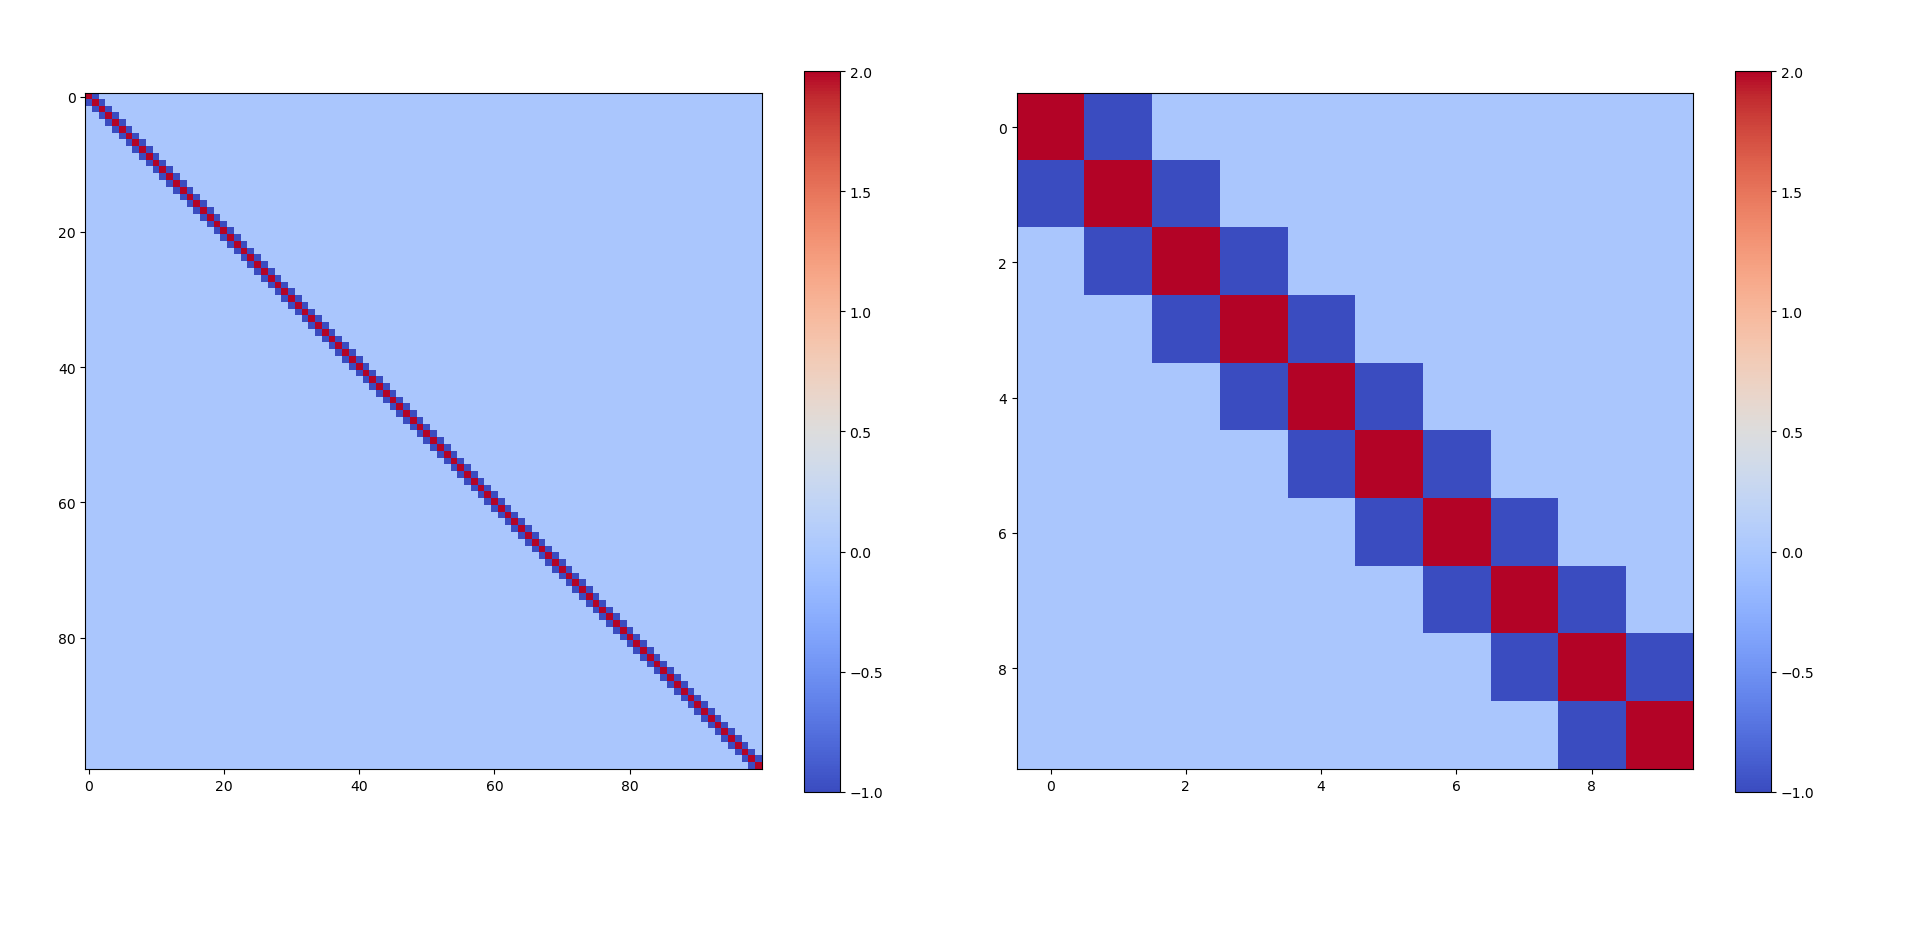
\includegraphics[width=15cm]{p1_1}
\caption{The Hamiltonian matrix for $t=1$}
\label{fig:method}
\end{figure}

\subsection{D}

The sorted eigenvalues are shown in Figure 1d.

\subsection{E}

\begin{figure}[t!]
\centering
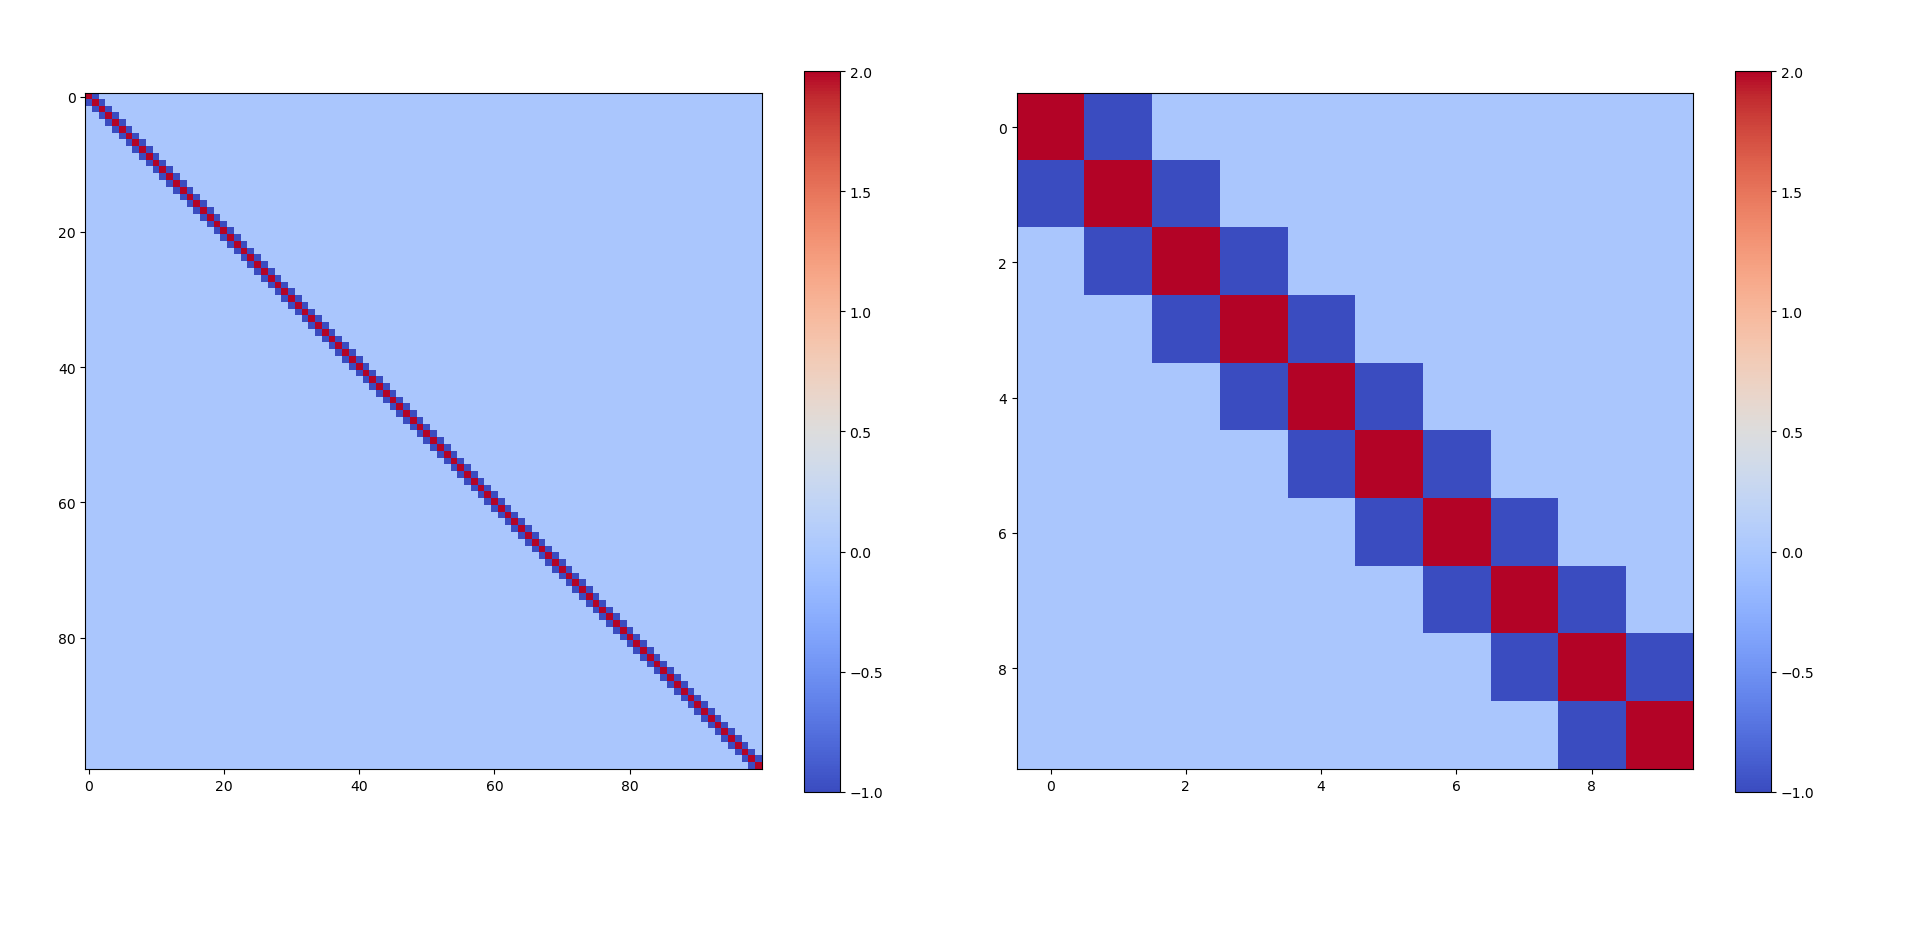
\includegraphics[width=15cm]{p1_1}
\caption{The Hamiltonian matrix for $t=1$}
\label{fig:method}
\end{figure}



\end{document}